\documentclass{article}

\usepackage{tikz}

\begin{document}
    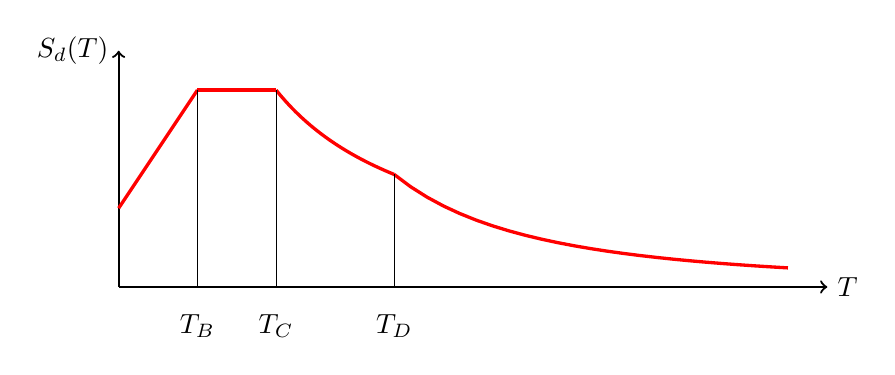
\begin{tikzpicture}
        
        \draw[->, black, thick] (0,0) -- (9,0) node[right] {$T$};
        \draw[->, black, thick] (0,0) -- (0, 3) node[left] {$S_d(T)$};
        
        
        \draw[domain = 0:1, red, very thick] plot(\x, 1.5 * \x + 1);
        \draw[domain = 1:2, red, very thick] plot (\x, 2.5);
        \draw[domain = 2:3.5, red, very thick] plot (\x, 5 / \x);
        \draw[domain = 3.5:8.5, red, very thick] plot (\x, 17.5 / \x^2);
        
        \node at (1,-0.5) {$T_B$};
        \draw[black, thin] (1, 0) -- (1, 2.5);
        
        \node at (2, -0.5) {$T_C$};
        \draw[black, thin] (2, 0) -- (2, 2.5);
        
        \node at (3.5, -0.5) {$T_D$};
        \draw[black, thin] (3.5, 0) -- (3.5, 1.43);
        
    \end{tikzpicture}
\end{document}